\section{Graphes connexes, eulériens et bipartis }
\subsection{Graphes}

\index{graphe}
\begin{mydef}
  Un \emph{graphe} est un triplet ($V$, $E$, $\varphi$), où :\\
  - $V$ est un ensemble dont les éléments sont appelés sommets ou noeuds; \\
  - $E$ est un ensemble dont les éléments sont appelés arêtes; \\
  - $\varphi$ est une fonction, dîte fonction d'incidence, qui associe à chaque arête un sommet ou une paire de sommets.
\end{mydef}

\index{sommets adjacents}
\begin{mydef}
  Deux sommets incidents à la même arête sont dits \emph{adjacents}.
\end{mydef}

\index{boucle}
\begin{mydef}
  Une arête incidente à un seul sommet est une \emph{boucle}.
\end{mydef}

\index{degré}
\begin{mydef}
  Le \emph{degré} d'un sommet est le nombre d'arêtes incidentes à celui-ci.
\end{mydef}

\index{graphe!sous-graphe}
\begin{mydef}
  Un \emph{sous-graphe du graphe} ($V$, $E$, $\varphi$) est un graphe ($V'$, $E'$, $\varphi'$) avec : \\
  - $V' \subseteq V$ ; \\
  - $E' \subseteq E$ ; \\
  - $\varphi'$ est la restriction de $\varphi'$ à $E'$.
\end{mydef}

\index{isomorphisme}
\subsection{Isomorphisme de Graphes}
\begin{mydef}
  Deux graphes ($V$, $E$, $\varphi$) et ($V'$, $E'$, $\varphi'$) sont dits \emph{isomorphes} s'il existe des bijections $f:V \to V'$ et $g:E \to E'$ telles que :
  \begin{center}
    $\varphi(e) = \{u, v\}$ ssi $\varphi(g(e)) = \{f(u), f(v)\}$.
  \end{center}
  Deux graphes sont isomorphes s'il y a une bijection entre les noeuds et les arêtes.
\end{mydef}

\begin{myexem}
  Voici deux exemples d'isomorphisme du même graphe :
    \begin{figure} [!h]
      \centering
	    \subfigure[]
    	{
    	  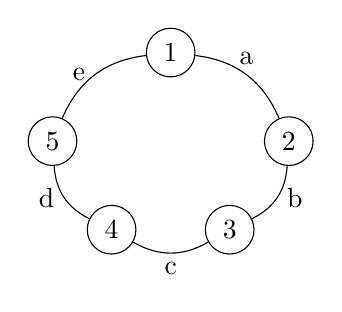
\begin{tikzpicture}[scale = 0.75]
          \node[draw, circle] at ( 0, 1.5)  (1) {1};
          \node[draw, circle] at ( 2, 0  )  (2) {2};
          \node[draw, circle] at ( 1,-1.5)  (3) {3};
          \node[draw, circle] at (-1,-1.5)  (4) {4};
          \node[draw, circle] at (-2, 0  )  (5) {5};

          \draw[-] (1) edge [bend left] node[anchor = south] {a} (2);
          \draw[-] (2) edge [bend left] node[anchor = west]  {b} (3);
          \draw[-] (3) edge [bend left] node[anchor = north] {c} (4);
          \draw[-] (4) edge [bend left] node[anchor = east]  {d} (5);
          \draw[-] (5) edge [bend left] node[anchor = east]  {e} (1);
        \end{tikzpicture}
      }
      % Cette ligne de commentaire semble être nécessaire pour que les figures soient affichées sur une ligne
      \subfigure[]
      {
        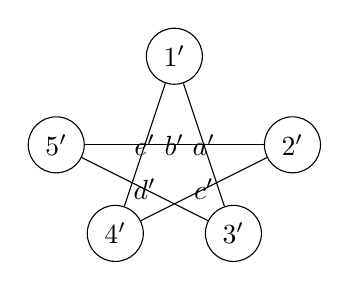
\begin{tikzpicture}[scale = 0.75]
          \node[draw, circle] at ( 0, 1.5)  (1) {$1'$};
          \node[draw, circle] at ( 2, 0  )  (2) {$2'$};
          \node[draw, circle] at ( 1,-1.5)  (3) {$3'$};
          \node[draw, circle] at (-1,-1.5)  (4) {$4'$};
          \node[draw, circle] at (-2, 0  )  (5) {$5'$};

          \draw[-] (1) edge node {$a'$} (3); %TODO mettre le label autrement pour que ce soit lisible
          \draw[-] (2) edge node {$b'$} (5); %TODO mettre le label autrement pour que ce soit lisible
          \draw[-] (2) edge node {$c'$} (4); %TODO mettre le label autrement pour que ce soit lisible
          \draw[-] (3) edge node {$d'$} (5); %TODO mettre le label autrement pour que ce soit lisible
          \draw[-] (1) edge node {$e'$} (4); %TODO mettre le label autrement pour que ce soit lisible

          %TODO tracer les lignes qui montrent comment on passe du graphe b au graphe c (en gardant les 3 graphes sur la même ligne)

        \end{tikzpicture}
      }
      % Cette ligne de commentaire semble être nécessaire pour que les figures soient affichées sur une ligne
      \subfigure[]
      {
        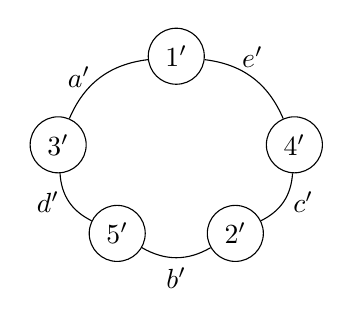
\begin{tikzpicture}[scale = 0.75]
          \node[draw, circle] at ( 0, 1.5)  (1) {$1'$};
          \node[draw, circle] at ( 2, 0  )  (4) {$4'$};
          \node[draw, circle] at ( 1,-1.5)  (2) {$2'$};
          \node[draw, circle] at (-1,-1.5)  (5) {$5'$};
          \node[draw, circle] at (-2, 0  )  (3) {$3'$};

          \draw[-] (1) edge [bend left] node[anchor = south] {$e'$} (4);
          \draw[-] (4) edge [bend left] node[anchor = west]  {$c'$} (2);
          \draw[-] (2) edge [bend left] node[anchor = north] {$b'$} (5);
          \draw[-] (5) edge [bend left] node[anchor = east]  {$d'$} (3);
          \draw[-] (3) edge [bend left] node[anchor = east]  {$a'$} (1);
        \end{tikzpicture}
      }
    \end{figure}
    Notons que les graphes \emph{b} et \emph{c} sont les mêmes, leurs noeuds ont simplement été réordonnés.\\
    L'isomorphisme entre \emph{a} et les deux autres est donné par : \\

    \begin{tabular}{lll}
      $f(1)=1'$ & $g(a)=e'$ \\
      $f(2)=4'$ & $g(b)=c'$ & $\varphi(a) = \{1, 2\}$\\
      $f(3)=2'$ & $g(c)=b'$ & $\varphi'(a') = \{1', 3'\}$\\
      $f(4)=5'$ & $g(d)=d'$ & $\varphi'(g(a)) = \{f(1), f(2)\}$\\
      $f(5)=3'$ & $g(e)=a'$ \\
    \end{tabular}
    \newline
    \newline
    Notons aussi que plusieurs résultats sont possibles : \\
    \begin{figure}[!h]
      \centering
      \subfigure[]
      {
        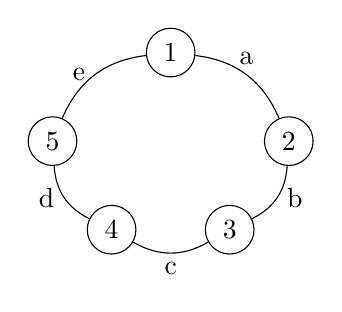
\begin{tikzpicture}[scale = 0.75]
          \node[draw, circle] at ( 0, 1.5)  (1) {1};
          \node[draw, circle] at ( 2, 0  )  (2) {2};
          \node[draw, circle] at ( 1,-1.5)  (3) {3};
          \node[draw, circle] at (-1,-1.5)  (4) {4};
          \node[draw, circle] at (-2, 0  )  (5) {5};

          \draw[-] (1) edge [bend left] node[anchor = south] {a} (2);
          \draw[-] (2) edge [bend left] node[anchor = west]  {b} (3);
          \draw[-] (3) edge [bend left] node[anchor = north] {c} (4);
          \draw[-] (4) edge [bend left] node[anchor = east]  {d} (5);
          \draw[-] (5) edge [bend left] node[anchor = east]  {e} (1);
        \end{tikzpicture}
      }
      % Cette ligne de commentaire semble être nécessaire pour que les figures soient affichées sur une ligne
      \subfigure[]
      {
        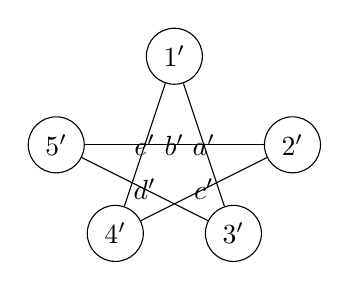
\begin{tikzpicture}[scale = 0.75]
          \node[draw, circle] at ( 0, 1.5)  (1) {$1'$};
          \node[draw, circle] at ( 2, 0  )  (2) {$2'$};
          \node[draw, circle] at ( 1,-1.5)  (3) {$3'$};
          \node[draw, circle] at (-1,-1.5)  (4) {$4'$};
          \node[draw, circle] at (-2, 0  )  (5) {$5'$};

          \draw[-] (1) edge node {$a'$} (3); %TODO mettre le label autrement pour que ce soit lisible
          \draw[-] (2) edge node {$b'$} (5); %TODO mettre le label autrement pour que ce soit lisible
          \draw[-] (2) edge node {$c'$} (4); %TODO mettre le label autrement pour que ce soit lisible
          \draw[-] (3) edge node {$d'$} (5); %TODO mettre le label autrement pour que ce soit lisible
          \draw[-] (1) edge node {$e'$} (4); %TODO mettre le label autrement pour que ce soit lisible

          %TODO tracer les lignes qui montrent comment on passe du graphe e au graphe f (en gardant les 3 graphes sur la même ligne)
        \end{tikzpicture}
      }
      % Cette ligne de commentaire semble être nécessaire pour que les figures soient affichées sur une ligne
      \subfigure[]
      {
        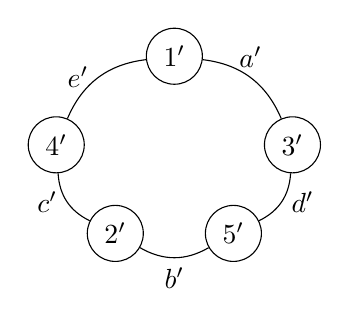
\begin{tikzpicture}[scale = 0.75]
          \node[draw, circle] at ( 0, 1.5)  (1) {$1'$};
          \node[draw, circle] at ( 2, 0  )  (3) {$3'$};
          \node[draw, circle] at ( 1,-1.5)  (5) {$5'$};
          \node[draw, circle] at (-1,-1.5)  (2) {$2'$};
          \node[draw, circle] at (-2, 0  )  (4) {$4'$};

          \draw[-] (1) edge [bend left] node[anchor = south] {$a'$} (3);
          \draw[-] (3) edge [bend left] node[anchor = west]  {$d'$} (5);
          \draw[-] (5) edge [bend left] node[anchor = north] {$b'$} (2);
          \draw[-] (2) edge [bend left] node[anchor = east]  {$c'$} (4);
          \draw[-] (4) edge [bend left] node[anchor = east]  {$e'$} (1);
        \end{tikzpicture}
      }
    \end{figure}

    \begin{tabular}{lll}
      $f(1)=1'$ & $g(a)=a'$ \\
      $f(2)=3'$ & $g(b)=b'$ \\
      $f(3)=5'$ & $g(c)=d'$ \\
      $f(4)=2'$ & $g(d)=c'$ \\
      $f(5)=4'$ & $g(e)=e'$ \\
    \end{tabular}
    \newline
    \newline
    Les six graphes de cet exemple sont isomorphes entre eux.
\end{myexem}

\subsection{Parcours eulérien}
\index{parcours}
\begin{mydef}%TODO définir ce qu'est un parcours
  Un \emph{parcours} est fermé si $v_0 = v_1$.
\end{mydef}

\index{chemin}
\begin{mydef}
  Un \emph{chemin} est un parcours dont tous les sommets sont distincts.
\end{mydef}

\index{cycle}
\begin{mydef}
  Un \emph{cycle} est un parcours fermé dont tous les sommets d'origine et intérieurs sont tous distincts.
\end{mydef}

\index{graphe!graphe connexe}
\begin{mydef}
  Un \emph{graphe} est \emph{connexe} si pour chaque pair de points il existe un parcours qui les relie. Les \emph{composantes connexes} d'un graphe sont ses sous-graphes connexes maximaux.
\end{mydef}

\index{parcours!parcours eulérien}
\index{graphe!graphe eulérien}
\begin{mydef}
  Un \emph{parcours} est \emph{eulérien} s'il visite chaque arête une et une seule fois. Un \emph{graphe} est \emph{eulérien} s'il existe un parcours eulérien fermé.
\end{mydef}

\begin{mytheo} [Théorème d'Euler]
  Un graphe connexe est eulérien ssi tous les sommets sont de degré pair.
  \begin{proof}
    \noindent
    \newline
    \fbox{$\Longrightarrow$}
    \newline
    Chaque arête incidente à un noeud $x$ est utilisé par le parcours eulérien:
    \begin{itemize}
      \item soit pour entrer dans $x$;
      \item soit pour en sortir.\\
    \end{itemize}
    A chaque arête entrante correspond une arête sortante (celle qui suit dans le parcours sauf pour la dernière et la première).\\
    Donc, il y a une bijection entre les arêtes entrantes et les arêtes sortantes.\\
    $\longrightarrow$ degré pair \\

    \noindent
    \fbox{$\Longleftarrow$}
    \newline
    On va construire un parcours un parcours eulérien :\\
    \begin{enumerate}
      \item On part d'un noeud arbitraire $x_0$.
      \item On prend une arête incidente à $x_0$, on arrive à un nouveau noeud.
      \item Par parité, il y a au moins une arête non utilisée, on la prend, etc... Quand il n'y a plus d'arête disponible, on est forcément arrivé à $x_0$.\\
    \end{enumerate}

    INSERT GRAPH HERE \href{https://dl.dropboxusercontent.com/u/44092863/Graph_Theory_Romain_Capron.pdf}{Voir notes} \addTODO\\

    Pour tout autre noeud y, en arrivant à y, on a utilisé un nombre impair d'arêtes incidentes à y. On a un parcours fermé :
    \begin{itemize}
      \item Si toutes les arêtes incidentes aux x noeuds traversés par ce parcours sont utilisées, alors ce parcours est eulérien;
      \item Sinon, il y a $x_1 \in$ parcours avec au moins une arête non exploitée.\\
    \end{itemize}

    INSERT GRAPH HERE \href{https://dl.dropboxusercontent.com/u/44092863/Graph_Theory_Romain_Capron.pdf}{Voir notes} \addTODO\\

    On merge les deux parcours :\\
    $P_{0+1} = x_0 \rightarrow x_1 \textcolor{red}{\rightarrow} x_1 \rightarrow x_0$\\
    Et on fait ça en boucle jusqu'à avoir toutes les arêtes.
  \end{proof}
\end{mytheo}

\begin{mytheo} [Existence d’un parcours eulérien]
  Un graphe connexe possède un parcours eulérien ssi le nombre de noeuds de degré impair est zéro ou deux.
  \begin{proof} In Progress
    \noindent
    \newline
    \fbox{$\Longrightarrow$}
    \newline
    \begin{itemize}
      \item ;
      \item .\\
    \end{itemize}

    \noindent
    \fbox{$\Longleftarrow$}
    \newline
  \end{proof}
\end{mytheo}

\begin{mytheo} [Théorème des poignées de mains]
  La somme des degrés des noeuds d’un graphe est deux fois le nombre d’arêtes.
  \begin{proof}
     \href{https://dl.dropboxusercontent.com/u/44092863/Graph_Theory_Romain_Capron.pdf}{Voir notes} \addTODO
  \end{proof}
\end{mytheo}

\subsection{Représentation matricielle du graphe}
\index{matrice d'adjacence}
\begin{mydef}
  La \emph{matrice d'adjacence} est une matrice carrée $n$x$n$ dont l'élément $ij$ est le nombre d'arêtes entre les sommets $v_i$ et $v_j$.
\end{mydef}

\index{matrice d'incidence}
\begin{mydef}
  La \emph{matrice d'incidence} est une matrice rectangulaire $n$x$m$ dont l'élément $ij$ est le nombre de fois que le sommet $v_i$ est incident à l'arête $e_j$.
\end{mydef}

\begin{myexem}
  \href{https://dl.dropboxusercontent.com/u/44092863/Graph_Theory_Romain_Capron.pdf}{Voir notes} \addTODO
\end{myexem}

\begin{mytheo} [Matrice d’adjacence et nombre de parcours]
  Soit $A$ la matrice d'adjacence d'un graphe. Alors l'élément $ij$ de $A^k$ ($k \geq 0$) est le nombre de parcours de longueur $k$ de $v_i$ vers $v_j$.
  \begin{proof}
     \href{https://dl.dropboxusercontent.com/u/44092863/Graph_Theory_Romain_Capron.pdf}{Voir notes} \addTODO
  \end{proof}
\end{mytheo}

\index{distance entre deux noeuds}
\begin{mydef}
  La \emph{distance $d(u, v)$} entre les noeuds $u$ et $v$ d'un graphe est le nombre d'arêtes minimal d'un parcours entre ces deux noeuds.
\end{mydef}

\begin{mylem}
  Si $u...u'...v'...v$ est un parcours de longeur minimale de $u$ vers $v$, alors le sous-parcours $u'...v'$ est un parcours de longeur minimale de $u'$ vers $v'$.\\
  En particulier, un parcours de longueur minimale est toujours un chemin.
  \begin{proof}
    Si ce parcours entre $u'$ et $v'$ n'était pas le plus court, on utiliserait le parcours strictement plus court pour la construction du parcours entre $u$ et $v$.
  \end{proof}
\end{mylem}

\subsection{Graphe biparti}
\index{graphe!graphe biparti}
\begin{mydef}
  Un graphe est \emph{biparti}  s'il existe une partition en deux ensembles $V_1$ et $V_2$ tels que les sommets de $V_1$ ne sont adjacents qu'à des sommets de $V_2$ et vice versa. La bipartition est $(V_1, V_2)$.
\end{mydef}

\begin{myexem}
  \href{https://dl.dropboxusercontent.com/u/44092863/Graph_Theory_Romain_Capron.pdf}{Voir notes} \addTODO
\end{myexem}

\begin{mytheo} [Graphes bipartis]
  Un graphe est biparti ssi tous ses cycles sont de longueur paire.
  \begin{proof}
     \href{https://dl.dropboxusercontent.com/u/44092863/Graph_Theory_Romain_Capron.pdf}{Voir notes} \addTODO
  \end{proof}
\end{mytheo}
